\documentclass[dvipdfmx]{jsarticle}
\usepackage[T1]{fontenc}
\usepackage[dvipdfmx]{hyperref}
\usepackage{lmodern}
\usepackage{latexsym}
\usepackage{amsfonts}
\usepackage{amssymb}
\usepackage{mathtools}
\usepackage{nccmath}
\usepackage{amsthm}
\usepackage{multirow}
\usepackage{graphicx}
\usepackage{wrapfig}
\usepackage{here}
\usepackage{float}
\usepackage{ascmac}
\usepackage{url}

\title{interface、抽象クラスを利用したJavaのペア・プログラミング課題}
\author{文理学部情報科学科\\5419045 高林 秀 5419071出川慎悟}
\date{\today}

\begin{document}

\maketitle

\begin{abstract}
  本稿では、今年度オブジェクト指向プログラミングの課題研究2として、前回の課題研究で制作したJavaプログラムを、パ−トナーのソースコードと統合し、加えてZoog以外の新しいキャラクターの描画を行うものである。本演習には、Javaを使用した。
  結果、課題1ではそれぞれのソースコード統合に成功し、呼び出し側の共通化もできた。課題2では、Zoogと見た目動作が異なるキャラクターを描画した。加えて、intefaceキーワードを利用することで、課題1でのZoogクラスの子クラスとの呼び出し側共通化もできた。
\end{abstract}

\section{目的}
本稿は、今年度オブジェクト指向プログラミングの課題研究として、Javaのペア・プログラミングを行うものである。今回の課題は、前回の課題研究1で作成したZoogクラスを、パートナーのJavaソースコードと統合すること、並びにZoogとは異なる形、動作をする新しいキャラクターを描画すること、である。その際、Zoogと同一のinterface等を利用し、呼び出し側を共通化する。

\section{課題概要}
本課題は下記に示す、2種類の課題から構成されている。以下にそれぞれの詳細を示す。\par
\begin{enumerate}
  \item 課題研究1で制作したプログラムを1つのプログラムに統合する。\par
  自分とパートナーの課題研究1で作成したZoogプログラムを比較し、1つのプログラムで呼び出しが行えるよう統合する。その際、共通の抽象クラスやinterfaceを利用するなど、適切な継承関係を与えること。
  \item 新しいキャラクターを追加する。\par
  Zoogと見た目、動き方、攻撃方法(なにをすると動きが止まるか)が異なる新しいキャラクターを描画する。その際、1で使用した抽象クラスやinterfaceを利用するなどし、呼び出し側を共通化することが望まれる。
\end{enumerate}
なお担当者は、1を出川慎悟、2を高林秀が担当した。
\section{設計方針}
\subsection{予備知識}
なお、今回制作した各クラスはZoog\_Objというパッケージでパッケージ化している。カプセル化やパッケージ化の基本的な解説は、本稿の前に執筆した課題研究1のレポートをご参照いただきたい。
\begin{itemize}
  \item Javaのカプセル化に関する課題研究:\url{https://drive.google.com/file/d/1UfX1tt-JeXKeJxtSKVJvA1OILJwYQsDd/view?usp=sharing}
\end{itemize}
なお、今回の課題研究ではJavaに備わっている機能であるinterface(インターフェイス)と抽象クラス(abstract class)呼ばれる機能を使用している。それについて少し説明する。
\subsubsection{interface(インターフェイス)}
抽象メソッドの宣言のみが行える。抽象メソッドには具体的な処理内容を記載しないため、変数とメソッドのデータ型のみを先に指定し、メソッドを利用する直前で処理内容を追加するといったことが可能になる。感覚的には継承を利用したメソッドのオーバーライドに近いと言えるだろう。\par
クラスの継承においては、継承元の親クラスは1つのみに限られるがinterfaceではその様な制限は無い。したがって、複数のinterfaceを継承するといった多重継承を行うこともできる。
interfaceの宣言は以下のように行う。
\begin{verbatim}
  interface "interfaceの名称" {
    void method1();
    int method2(int a, int b)
    .....
  }
\end{verbatim}
宣言したintefaceを実装するには、実装したいクラスでimplementsキーワードを利用する。
\begin{verbatim}
  class クラス名 implements "interfaceの名称" {
    //...コンストラクタやクラス変数の宣言等

    void method1() {
      //具体的な処理内容
    }
    int method2(int a, int b) {
      //具体的な処理内容
    }
    ....
  }
\end{verbatim}
\subsubsection{抽象クラス(abstract class)}
抽象メソッドを1つ以上有するクラスを抽象クラスと呼ぶ。抽象クラスは、継承先の小クラスにてメソッドのオーバーライドができるという特徴を持つ。抽象クラス記載時にはどの様な処理にするか決まっていないときでも、いずれ使用するメソッドを予め抽象メソッドとして宣言し、継承先の子クラスで処理内容を記載する、といった使い方ができる。\par
抽象クラスを宣言するには、abstractキーワードを使用する。
\begin{verbatim}
  abstract class "クラス名" {
    //...コンストラクタやメソッド、クラス変数の宣言等
    abstract void method1();
  }
\end{verbatim}

前章で示した各課題ごとに対する設計方針をまとめる。
\begin{enumerate}
\item 課題1\par
高林のプログラムにZoogクラスとそれを継承したSecondZoogクラスの二つがあり、出川のプログラムもそれに類似した内容だったのでその二つをまとめることを考える。ZoogクラスをHorizontalZoogクラスという名前にし、HorizontalZoogクラスとSecondZoogクラスの上に抽象クラスであるZoogクラスを作成しmoveメソッドを抽象メソッドとする。そして二つのクラスがZoogクラスを継承し、moveメソッドをオーバーライドすることで異なる動きをする2つのZoogを作成する。
\item 課題2\par
課題2も、指定された位置に特定の図形を描画しそれを動かすという意味では、課題1で作成したZoogと同じである。そこで、新たにZoogクラスと、新しいキャラクターのクラスを統合するCharactorと呼ばれるinterfaceを作成し、呼び出し側の共通化を図る。そのinterfaceをimplementsしたNewCaractorクラスそ作成し、その中で見た目、動き方、攻撃方法を定義している。なお動き方に関しては、既存のZoogクラス系のオブジェクトでは、ウィンドウの端で跳ね返り、上下左右に移動するもの、ただ単に左右に移動するもの、の2種類となっている。そこで、新しいキャラクターはウィンドウの左端に到達するまで高速で右端から左端に移動する、といった動作を考えた。
\end{enumerate}
\section{ソースコード}
課題1,課題2で作成したクラス、interfaceのコードを以下に示す。動作に必要なすべてのソースコードは巻末付録に添付しているGoogleDriveあるいはGitHubからダウンロードいただきたい。なお、統合前の課題研究1の高林、出川が制作したソースコードに関しては、以下のリンク、または巻末付録を参照いただきたい。
\begin{itemize}
  \item 課題研究1のコードリンク
  \begin{itemize}
    \item 高林:\url{https://drive.google.com/drive/folders/1ps_D8L_N2Nop4T_83lSPCHH4DMtAHr_t?usp=sharing}
    \item 出川:\url{https://drive.google.com/drive/folders/1La_4gfzS55Z_cNiKYDnXIuMV_sfyyhPb?usp=sharing}
  \end{itemize}
\end{itemize}
\begin{enumerate}
  \item 課題
  \begin{itemize}
    \item Zoog.java
    \begin{verbatim}
      package myprogram.Zoog_Obj;
      import processing.core.*;

      abstract class Zoog implements Charactor{
          public PApplet p;
          protected float x, y;
          protected float mx, my;
          protected int colorBW;
          protected boolean rightEye = true;
          protected boolean leftEye = true;

          public Zoog(PApplet pa) {
              p = pa;
              x = p.random(100, 200);
              y = p.random(100, p.height / 2);
              mx = p.random(1, 3);
              my = p.random(1, 3);

          }

          public void draw() {

              //zoog body
              p.stroke(0);
              p.fill(colorBW);
              p.rect(x, y, 20, 100);
              //zoog head
              p.fill(colorBW);
              p.ellipse(x, y-30, 60, 60);
              //zoog eye
              p.fill(0);
              if(leftEye == true) {
                p.ellipse(x-19, y-30, 16, 32);
              }
              if(rightEye == true) {
                p.ellipse(x+19, y-30, 16, 32);
              }
              p.fill(0);
              //zoog leg
              p.stroke(0);
              p.line(x-10, y+50, x-20, y + 60);
              p.line(x+10, y+50, x+20, y + 60);
          }

         //public void move();//抽象メソッド

         /*
          public void move() {//zoogを動かすメソッド
              if(x + 20 >= p.width + 20 || x < 0) {//zoogがウィンドウの端に来た際に跳ね返る動作を行う
                  mx *= -1;
              }
               x += mx;//zoogを動かす

              if(leftEye == false && rightEye == false) {
                 mx = 0;
              }
          }
         */

          public void judgeClick(int MouseX, int MouseY) {
          if( (MouseX > x-27 &&  MouseX < x-11)  && (MouseY > y-46 && MouseY < y-14) ) {
            leftEye = false;
          }
          if( (MouseX > x+11 && MouseX < x+27) && (MouseY > y-46 && MouseY < y-14) ) {
            rightEye = false;
          }
        }

         public boolean isInRange(int MouseX, int MouseY) {
            return (p.dist(MouseX, MouseY, x-19, y-30) < 16 || p.dist(MouseX, MouseY, x-19, y-30) < 40 ) ;
         }
      }
    \end{verbatim}
    \item SecondZoog.java
    \begin{verbatim}
      package myprogram.Zoog_Obj;

      import processing.core.*;

      public class SecondZoog extends Zoog{
          public SecondZoog(PApplet pa) {
              super(pa);
              colorBW = 255;
          }
          @Override
          public void move() {//moveメソッドをオーバーライドする
              if(x < 10 || x > p.width) {
                  mx *= -1;
              }
              if(y < 50 || y > p.height - 55) {
                  my *= -1;
              }
              x += mx;//zoogを動かす
              y += my;
              if(leftEye == false && rightEye == false) {
                 mx = 0;
                 my = 0;
              }
          }
      }
    \end{verbatim}
    \item HorizontalZoog.java
    \begin{verbatim}
      package myprogram.Zoog_Obj;

      import processing.core.*;

      public class HorizontalZoog extends Zoog {
         public HorizontalZoog(PApplet pa) {
            super(pa);

            colorBW = (int)p.random(1, 255);
         }

          public void move() {//moveメソッドをオーバーライドする
              if(x + 20 >= p.width + 20 || x < 0) {//zoogがウィンドウの端に来た際に跳ね返る動作を行う
                  mx *= -1;
              }
               x += mx;//zoogを動かす

              if(leftEye == false && rightEye == false) {
                 mx = 0;
              }
          }

      }
    \end{verbatim}
  \end{itemize}
  \item 課題2 
  \begin{itemize}
    \item Charactor.java 
    \begin{verbatim}
      package myprogram.Zoog_Obj;

      interface Charactor {
          void draw();
          void move();
          void judgeClick(int MouseX, int MouseY);
          boolean isInRange(int MouseX, int MouseY);
      }
    \end{verbatim}
    \item NewCharacotr.java
    \begin{verbatim}
      package myprogram.Zoog_Obj;
      import processing.core.*;

      public class NewCharactor implements Charactor{

          private PApplet p;
          private boolean moving = true;
          private boolean draw_text = false;
          private float x, y, mx;
          private boolean rightEye = true;
          private boolean leftEye = true;


          public NewCharactor(PApplet pa) {
              //super(pa);
              p = pa;
              x = p.random(100, 200);
              y = p.random(100, p.height / 2);
              mx = p.random(1, 3);
              //my = p.random(1, 3);
          }

          public void draw() {
              //body
              p.fill(190);
              p.rect(x, y, 100, 20);
              //head
              p.fill(100);
              p.ellipse(x-30, y, 60, 60);
              //eye
              p.fill(0);
              if(leftEye) {
                  p.ellipse((x-30)-10, y, 15, 20);
              }
              if(rightEye) {
                  p.ellipse((x-30)+10, y, 15, 20);
              }
              if(draw_text) {
                  displayText("HEY!!Mr.Kitahara!!.How are you ??.", 60);
              }
              //leg
              //p.line(x+10, y+20, (x+50)-20, (y+20)+40);
              //p.line(x+40, y+20, (x+50)+20, (y+20)+40);
          }

          public void move(){
              if(moving) {
                  if(x <= 0) {
                      x = p.width;
                  } else {
                      x -= 3 * mx;
                  }
              }
          }

          private void displayText(String text, int size) {
              p.textAlign(p.CENTER);
              p.textSize(size);
              p.fill(170, 20, 20);
              p.text(text, x, y + 20);
          }
          public boolean isInRange(int MouseX, int MouseY){
              return (p.dist(MouseX, MouseY, x-19, y-30) < 16 || p.dist(MouseX, MouseY, x-19, y-30) < 40 ) ;
          }

          public void judgeClick(int MouseX,int MouseY) {
              mx = 0;
              draw_text = true;
          }
      }
    \end{verbatim}
  \end{itemize}
\end{enumerate}
なお、今回のディレクトリ構成は以下の通りとなっている。・・・.javaはJavaファイルを、.javaが添付されていない名称はフォルダを示す。
\begin{itemize}
  \item Report2
  \begin{itemize}
    \item MyApplet.java
    \item myprogram
    \begin{itemize}
      \item Zoog\_Obj
      \begin{itemize}
        \item Charactor.java
        \item Zoog.java
        \item HorizontalZoog.java
        \item SecondZoog.java
        \item NewCharacotr.java
      \end{itemize}
    \end{itemize}。
  \end{itemize}
\end{itemize}
起動するには、親ディレクトリReport2に存在するMyApplet.javaをコンソールで呼び出して起動する。
\section{実行結果}
以下、MyApplet.java起動時の結果を示す。
\subsection{結果のスクリーンショット}
\begin{figure}[H]
  \centering
  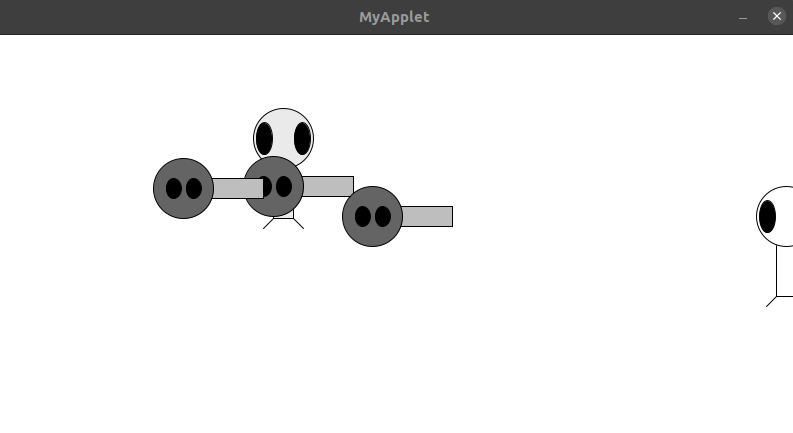
\includegraphics[scale=0.4]{images/result1.png}
  \caption{実行時の画像1}
\end{figure}
\begin{figure}[H]
  \centering
  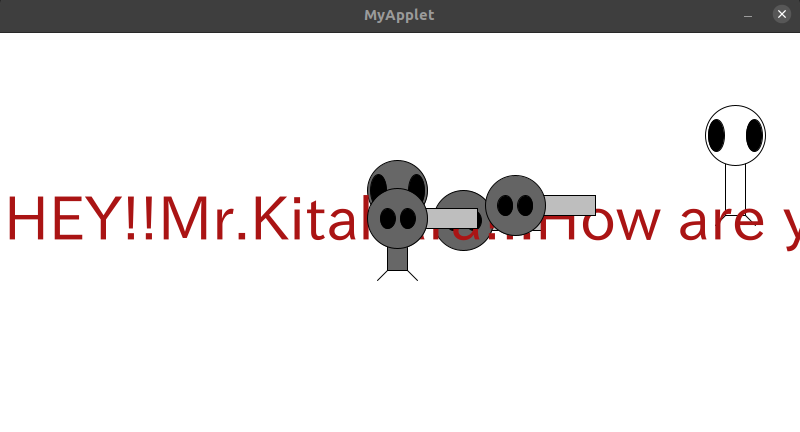
\includegraphics[scale=0.4]{images/result2.png}
  \caption{実行時の画像2}
\end{figure}
\begin{figure}[H]
  \centering
  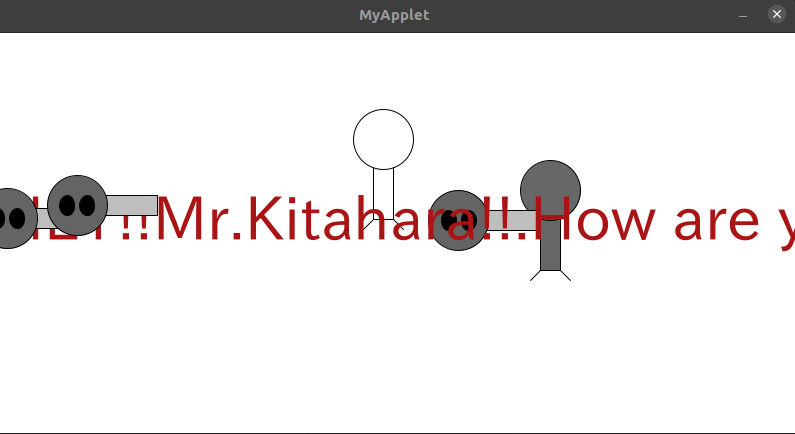
\includegraphics[scale=0.4]{images/result3.png}
  \caption{実行時の画像3}
\end{figure}
\subsection{結果の説明}
起動直後、2体のZoogと、3体の新しいキャラクターが描画される※画像1。なお出現位置は、$x$座標が100以上200未満の間でランダムに、$y$座標が100以上ウィンドウの高さ$\div 2$未満の間でランダムに決定する。\par
Zoogは左右に移動しウィンドウの端に到達すると跳ね返るものと、上下左右に移動しウィンドウの端で跳ね返るもの、の2種類の動作をする。眼の部分をマウスでクリックすると、眼が消滅するようになっており、両目を消失するとそのZoogの動作が止まるようになっている※画像3。\par
3体の新しいキャラクター(以降NewFishと呼称する)は、ウィンドウ右端から左端へ高速に移動している。
なお、3体のうち1体の、頭をクリックすると、その動作が停止しウィンドウ上に"HEY!!Mr.Kitahara!!.How are you ??."の文字列を描画する※画像2。その他2体はクリックしても、動作が停止しないようになっている(プログラム実行時に、どのZoogFishが文字列を出力するか当てて見てほしい)。\par
なお、実行時の動画を下記のURLに掲載する。
\begin{itemize}
  \item 動画リンク:\url{https://drive.google.com/file/d/12epGAvaELqIP-hwvUmeL9nQ_mFHwg4Rj/view?usp=sharing}
\end{itemize}
\section{考察}
今回は、先に示したとおり、以下に示す2つが達成目標となるだろう。
\begin{itemize}
  \item 高林と出川の課題研究1で作成したコードの統合
  \item NewFishの制作と、Zoogと呼び出し側の共通化
\end{itemize}
まず、2人のコードの統合の方について考察する。設計方針でも述べたが、Zoogクラスを抽象クラスにし、HorizontalZoogおよびSecondZoogクラスは、親クラスであるZoogを継承する形を取っている。抽象クラスを用意し、子クラスにそれを継承させることで、子クラスにコードが分散するのを防ぐことができる他、親クラスである抽象クラスを見れば、子クラスにどの様なメソッドがあるのか、またそのメソッドがどの様な動作をするのかということが容易に把握できる。加えて、抽象メソッドを定義することで、それぞれの子クラスの違いの把握や、メソッド名を統一することができ、呼び出し側の共通化を図ることができる。したがってプログラム全体の可読性の向上に繋がる。今回制作したコードは、前述の抽象クラスを継承する形を取っているので、可読性は高いと判断できる。加えて、子クラスに共通する部分(例えば今回の例ではZoogクラスのdraw()メソッドがそれに該当する)を変更したい時、クラスの継承を利用すれば、親クラスでの変更がそのまま子クラスに適用できるので、コードの拡張性という観点からも良いと言えるであろう。また、統合後動作で特に意図しない様な動作やエラー等も見られなかった。\par
次に、NewFishの制作の方について考察する。こちらは課題1とは異なり、Zoogクラスを継承させていない。あくまでもZoogとは別のオブジェクトであるので、Zoogクラスを継承し、メソッドをオーバーライドすることで既存のZoogと異なる見た目、動作を実現するといった方式は取らなかった。クラス継承のデメリットとして、無計画に継承を利用するとコードを単に分散させるだけになってしまう他、クラス間の関係性を強くする特性を持つので、やみくもに継承を利用するのは保守性、可読性の観点から望ましくない。その他、親クラスに抽象メソッド以外のメソッドや変数を書かれてしまう可能性があるのに加え、子クラスが多数に及ぶ場合、親クラスのコード修正の影響がそのすべての子クラスに影響を与えてしまう。そうすると、予期しないエラーや動作が起こるといった危険がある。つまり、呼び出し側の共通化のみが目的であれば、継承を利用するのはあまり望ましいとは言えない。今回制作したNewFishは、設計方針でも述べたように機能的にはZoogと同等であるが。、全くの別物である。したがってNewFish制作においては、Charactorと言う名称のinterface(以降Charactorインターフェイスと呼称する。)を用意し、NewFishの実装を行っているNewCharacotrクラスにimplementsさせている。このCharactorインターフェイスは、SecondZoog、HorizontalZoogクラスの継承元である抽象クラスZoogにもimplementsされている。このようにすることで、Zoogクラスを継承せずとも、呼び出し側でZoogクラスとその子(派生)クラスとの呼び出し共通化を実現することができた。加えて、ZoogクラスとNewCharactorクラスのクラス間の独立性を保つこともできた。\par
最後に、呼び出し側であるMyApplet.javaの記載を見るとメソッド呼び出しの共通化がなされているのが確認できる。よって、課題1,課題2の目標を達成したと言えるだろう。\par
余談だが、interfaceにももちろんデメリットは存在する。例えば、interfaceで宣言されたメソッドには処理を記載することができないため、同じ様な処理内容でも逐次各クラス記述しなければならないといったデメリットも存在する。したがって、使用法が適切でないとかえってコードの重複が増えることになり、冗長性が増してしまう。
\section{まとめ}
本稿では今年度オブジェクト指向プログラミングの課題研究2として、Javaでのペア・プログラミングを行った。内容は、課題研究1で作成したJavaプログラムを、1つのJavaプログラムに統合すること、並びに新たなキャラクターを制作し統合したZoogクラスと呼び出し側の共通化を図ることであった。全体的な結果としては、プログラムが正常に動作しているのでコードの統合はうまく行っていると言って良いだろう。
\section{各メンバーの貢献内容}
\begin{itemize}
  \item 高林秀
  \begin{itemize}
    \item 課題2の企画設計、コーディング担当。レポートの執筆。
  \end{itemize}
  \item 出川慎悟
  \begin{itemize}
    \item 課題1の企画設計、コーディング担当。課題2の設計考案。
  \end{itemize}
\end{itemize}
\section{巻末付録}
本稿で使用している画像ファイルや、Javaファイルは以下のアドレスから入手することができる。必要に応じてダウンロードいただきたい。
\begin{itemize}
  \item GoogleDrive:\url{https://drive.google.com/drive/folders/1QEt-NBptDGq2J1BgOyFnGUx8SMwL5oNc?usp=sharing}
  \item GitHubリポジトリ:\url{https://github.com/tsyu12345/OOP-report2}
\end{itemize}


\end{document}
